\documentclass[tikz,border=10pt]{standalone}
\usetikzlibrary{arrows.meta, positioning, calc, decorations.pathreplacing, fit}
\usepackage{amsmath}
\usepackage{amssymb}

\begin{document}
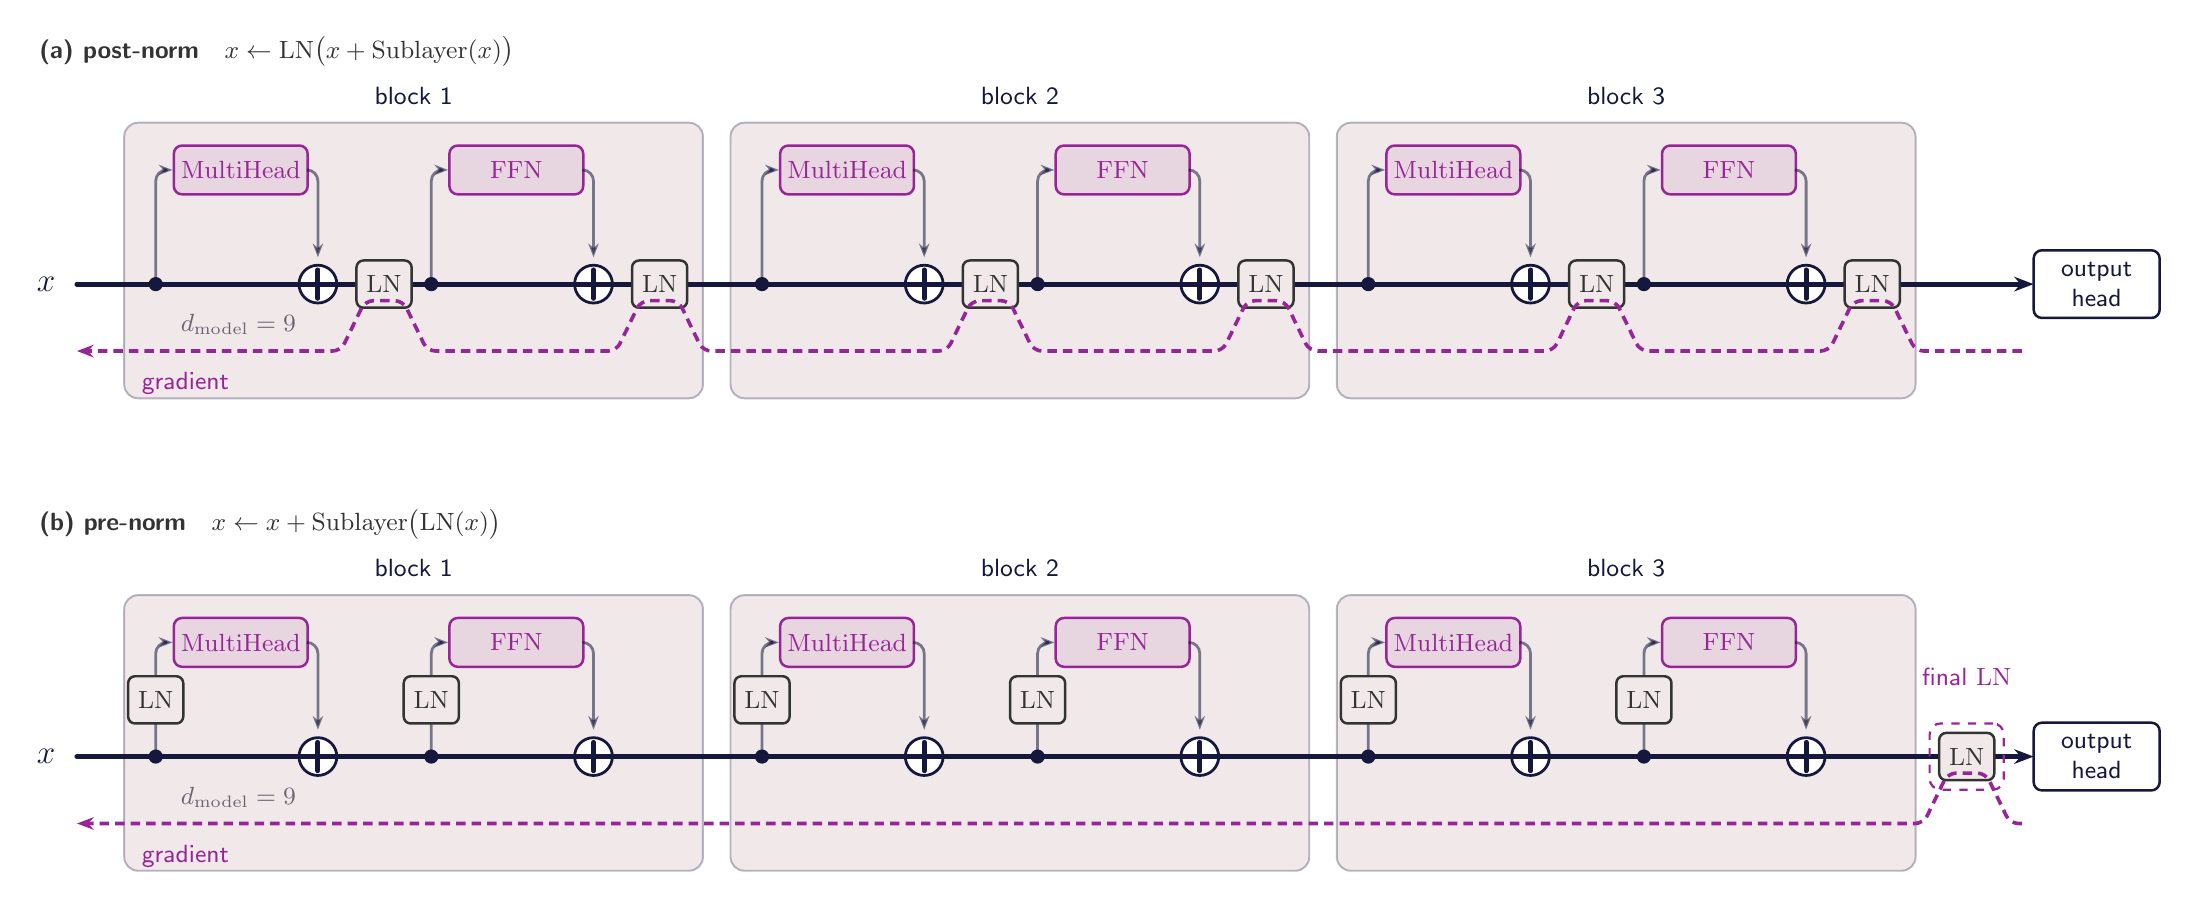
\begin{tikzpicture}[
    every node/.style={font=\sffamily},
]

\definecolor{c1}{HTML}{15173D}
\definecolor{c2}{HTML}{982598}
\definecolor{c3}{HTML}{E491C9}
\definecolor{c4}{HTML}{F1E9E9}
\definecolor{axiscolor}{HTML}{333333}
\definecolor{labelcolor}{HTML}{6B6472}

% ================================================================
% PLAN.  Two rows, each one variant, drawn by ONE skeleton macro so
% every element except the LN boxes is guaranteed identical.
%
% Local coordinates inside a row, y = 0 is the residual stream.
%
%   unit i taps the stream at x = T_i, pitch 3.50 inside a block,
%   extra 0.70 between blocks:
%     T = 0, 3.50, 7.70, 11.20, 15.40, 18.90
%     riser up at  T          to y = 1.45
%     sublayer box centred (T + 1.08, 1.45), 1.70 x 0.62
%     riser down at T + 2.06  to the add at (T + 2.06, 0)
%   sublayers alternate MultiHead, FFN; two per block, three blocks.
%
%   THE ADD, one construction everywhere in this section:
%     circle r = 0.24, white fill, c1 stroke 1.0pt; then the stream is
%     re-stroked straight across the circle at its own 2.4pt weight so
%     it is the horizontal bar of the plus and is never cut; then the
%     vertical stroke, c1 2.4pt, half-length 0.18.  No glyph text.
%
%   THE ONE DISPLACED BOX
%     post-norm : LN on the stream at (T_i + 2.90, 0)      i = 0..5
%     pre-norm  : LN on the riser   at (T_i,       0.72)   i = 0..5
%   nothing else moves.
%     clearances in (a): add edge T+2.30 | LN T+2.55..T+3.25 | tap T+3.50
%
%   block panels  x: -0.40..6.95 | 7.30..14.65 | 15.00..22.35
%                 y: -1.45..2.05,  label at y = 2.16
%   stream        x: -1.00..23.85,  output head box at 24.65
%   gradient      y = -0.85, running right to left and drawn last, so
%                 where it bumps up to y = -0.21 it is visibly threaded
%                 through the LN box rather than stopped under it:
%                 post-norm 2.90 6.40 10.60 14.10 18.30 21.80  (six)
%                 pre-norm  23.00 only, the final LN           (one)
%
%   rows: post-norm at y = 6.0, pre-norm at y = 0, titles at yb + 2.95
% ================================================================

\tikzset{
  stream/.style={c1, line width=1.8pt, line cap=round},
  branch/.style={c1, opacity=0.55, line width=1.0pt, rounded corners=4pt,
                 -{Stealth[length=5pt]}},
  sub/.style={draw=c2, line width=0.9pt, fill=c2, fill opacity=0.10,
              text opacity=1, text=c2, rounded corners=3pt,
              minimum width=1.70cm, minimum height=0.62cm, inner sep=1pt,
              font=\sffamily\small},
  ln/.style={draw=axiscolor, line width=0.9pt, fill=c4, text=axiscolor,
             rounded corners=2.5pt, minimum width=0.70cm,
             minimum height=0.60cm, inner sep=1pt, font=\sffamily\small},
  grad/.style={c2, line width=1.3pt, dash pattern=on 3.4pt off 2.2pt,
               rounded corners=3pt, -{Stealth[length=6pt]}},
  panel/.style={fill=c4, draw=c1, draw opacity=0.30, line width=0.7pt,
                rounded corners=5pt},
  blab/.style={font=\sffamily\small, text=c1, anchor=south},
  ann/.style={font=\sffamily\small, text=labelcolor},
  title/.style={font=\sffamily\small, text=axiscolor, anchor=west},
}

% the add: stream passes straight through, so the identity path is
% never broken by a white fill.  Argument: the x of the circle centre.
\newcommand{\addcirc}[1]{%
  \draw[draw=c1, line width=1.0pt, fill=white] (#1, 0) circle (0.24);
  \draw[stream] ({#1 - 0.25}, 0) -- ({#1 + 0.25}, 0);
  \draw[stream] (#1, -0.18) -- (#1, 0.18);
}

% ---------------------------------------------------------------- skeleton
% everything both variants share, drawn identically in both rows
\newcommand{\rowpanels}{%
  \foreach \a/\b/\n in {-0.40/6.95/1, 7.30/14.65/2, 15.00/22.35/3} {
      \path[panel] (\a, -1.45) rectangle (\b, 2.05);
      \node[blab] at ({0.5*(\a+\b)}, 2.16) {block \n};
  }
}
\newcommand{\rowbody}{%
  \draw[stream, -{Stealth[length=7pt]}] (-1.0, 0) -- (23.85, 0);
  \node[font=\sffamily\large, text=c1, anchor=east] at (-1.15, 0) {$x$};
  \node[ann, anchor=north] at (1.05, -0.26) {$d_{\mathrm{model}} = 9$};
  \foreach \i/\T/\nm in {0/0/MultiHead, 1/3.50/FFN, 2/7.70/MultiHead,
                         3/11.20/FFN, 4/15.40/MultiHead, 5/18.90/FFN} {
      \pgfmathsetmacro{\Tb}{\T + 2.06}
      \fill[c1] (\T, 0) circle (0.09);
      \node[sub] (s\i) at ({\T + 1.08}, 1.45) {$\mathrm{\nm}$};
      \draw[branch] (\T, 0) -- (\T, 1.45) -- (s\i.west);
      \draw[branch] (s\i.east) -- (\Tb, 1.45) -- (\Tb, 0.34);
      \addcirc{\Tb}
  }
  \node[draw=c1, line width=0.9pt, fill=white, rounded corners=3pt,
        minimum width=1.60cm, minimum height=0.86cm, align=center,
        text=c1, font=\sffamily\small] at (24.65, 0) {output\\head};
  \node[font=\sffamily\small, text=c2, anchor=north west] at (-0.30, -1.00)
      {gradient};
}

% ================================================================
% (a)  post-norm : the LN boxes sit ON the stream
% ================================================================
\begin{scope}[shift={(0, 6.0)}]
  \rowpanels
  \rowbody
  \foreach \T in {0, 3.50, 7.70, 11.20, 15.40, 18.90} {
      \node[ln] at ({\T + 2.90}, 0) {$\mathrm{LN}$};
  }
  \draw[grad] (23.70, -0.85)
      \foreach \c in {21.80, 18.30, 14.10, 10.60, 6.40, 2.90} {
        -- ({\c + 0.55}, -0.85) -- ({\c + 0.24}, -0.21)
        -- ({\c - 0.24}, -0.21) -- ({\c - 0.55}, -0.85) }
      -- (-1.0, -0.85);
  \node[title] at (-1.60, 2.95)
      {\textbf{(a) post-norm}\quad
       $x \leftarrow \mathrm{LN}\bigl(x + \mathrm{Sublayer}(x)\bigr)$};
\end{scope}

% ================================================================
% (b)  pre-norm : the same LN boxes, lifted onto the branches
% ================================================================
\begin{scope}[shift={(0, 0)}]
  \rowpanels
  \rowbody
  \foreach \T in {0, 3.50, 7.70, 11.20, 15.40, 18.90} {
      \node[ln] at (\T, 0.72) {$\mathrm{LN}$};
  }
  % the one extra box: the final LN, after the stack, before the head
  \node[ln] (fln) at (23.00, 0) {$\mathrm{LN}$};
  \node[draw=c2, dashed, line width=0.8pt, rounded corners=4pt,
        fit=(fln), inner sep=3pt] {};
  \node[font=\sffamily\small, text=c2, anchor=south] at (23.00, 0.78)
      {final $\mathrm{LN}$};
  \draw[grad] (23.70, -0.85)
      \foreach \c in {23.00} {
        -- ({\c + 0.55}, -0.85) -- ({\c + 0.24}, -0.21)
        -- ({\c - 0.24}, -0.21) -- ({\c - 0.55}, -0.85) }
      -- (-1.0, -0.85);
  \node[title] at (-1.60, 2.95)
      {\textbf{(b) pre-norm}\quad
       $x \leftarrow x + \mathrm{Sublayer}\bigl(\mathrm{LN}(x)\bigr)$};
\end{scope}

\end{tikzpicture}
\end{document}
